\section{Related Work and background} \label{sec:rel_work}
In the following, we will explain relevant sport theory concepts that our work is based upon and compare our approach to related research.
%\begin{itemize}
%	\item Put your work in the context of the related research in the field.
%	\item Summarize related literature and the relationship between the related work.
%	\item Identify missing parts in current research or missing opportunities in applying related work.
%	\item Reference possible future work of other papers to support your work, e.g.: \cite{bruegge2009object}.
%	\item Judge existing reproach by its reproducibility and credibility.
%	\item Do not just cite for the number of citations, each citation should have its justification your can defend if needed.
%\end{itemize}
\subsection{Sports theory background}\label{sec:sport_theory}
There are three different ways of energy provision in the muscles. The first and most efficient energy production comes from ATP that is stored in the cells. However, this only works for about 2 seconds. When this storage is depleted, the body generates ATP from glycogen that is also stored in the muscle cells. This way of energy provision is also very efficient but does not last for long, either. The long-time energy is produced by consuming oxygen (aerobic energy production) \cite{Bompa.2018}. Figure \ref{fig:energy_provision} shows how the energy in
the muscle cells is provided over time.  In the first seconds, the energy comes from the ATP stored in the muscle cells, and the anaerobic energy production starts.  The longer the activity lasts, the more energy comes from aerobic production. 50m sprints last for about 25s to 50s thus more than 60\% of the energy comes from anaerobic energy production \cite{Dr.PatriziaMayerHaralOchwatweitereBSVDozenten.2007} . As this energy production is independent of oxygen and its transport, the energy provision is independent of fatigue; thus, the 50m times in training are close to those in competition. This is an important fact on which we base our assumption that we can simulate the 50m times in training.
\begin{figure}[ht]
    \centering
    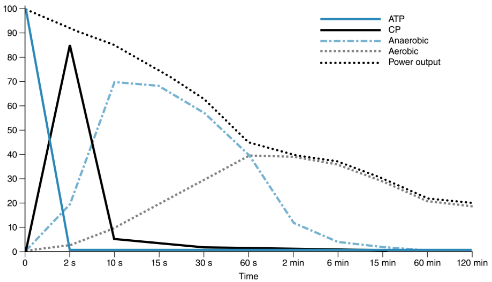
\includegraphics[scale=0.5]{visualisation/energy_provision.png}
    \caption{Energy provision by time \cite{Bompa.2018}}
    \label{fig:energy_provision}
\end{figure}
In general, a single training session can be split into multiple phases. During and shortly after the training session, the athlete is fatigued. After the training session has ended, the recovery starts. Recovery includes restoring energy stores in the muscles and reduce the lactic acid in the blood circulation. After many training sessions, the athlete's body starts to adapt to the constant exertion, i.e. the energy stores in the muscles increase and the heart muscle becomes stronger. This adaption process leads to improvement of the athlete's performance \cite{Bompa.2018.adaption}. Figure \ref{fig:training_improvement} visualises this adaption effect. The blue curve shows the performance of the athlete. With every stimulus, i.e. training session, the performance reduces to a minimum due to fatigue. After recovery, the maximum performance increases due to adaption. In this paper, we assume that athletes that have been training for a longer time perform better in competition. This assumption is based in the adaption process in the athlete's body.
\begin{figure}[ht]
    \centering
    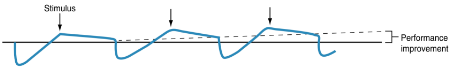
\includegraphics[scale=0.7]{visualisation/training_improvement.png}
    \caption{Performance improvement by continuous training \cite{Bompa.2018.compensation}}
    \label{fig:training_improvement}
\end{figure}
\subsection{Critical power concept} \label{critical_power}
In sports theory, critical power is the maximum rate that can be sustained for a very long time without fatigue \cite{Monod.1965,Hill.1993}. \citet{Monod.1965} introduced this concept and showed in their study that muscle power output and time to exhaustion follows a hyperbolic relationship while the total work performed is linearly connected to the time to exhaustion. Therefore, the critical power can be used as an indicator of the athlete's endurance and anaerobic capacity. With this indicator, coaches can optimise their training by setting loads and intensity in the aerobic area and evaluating the athlete's anaerobic performance without employing expensive material \cite{Dekerle.2002}. As \citet{Wakayoshi.1992} have shown  that these concepts are applicable for swimming in general. Moreover, \citet{Hill.1995} proved the applicability even for junior swimmers . The critical power concept is of interest for our work as it gives us an idea of how the distances and the corresponding times are related.
\subsection{Machine learning for swim result prediction}
To the best of our knowledge, there is no related work that uses the same approach as we propose. However, some papers use similar data representation or try to achieve the same result but based on a different setting.\\
\citet{Silva.2007} use neural nets to predict the swimmer’s performance in 200m individual medley and 400m freestyle based on how the swimmer performs in multiple fitness, strength and flexibility tests. The authors submitted 138 junior swimmers of national level to four test categories: kinanthropometric, general functional and specific functional tests as well as an evaluation of their swimming technique. With the results of these tests, they predict the swimmer’s competition performance using Artificial neural nets. Moreover, they determine the physical factors that affect this performance the most. Although the ground truth, i.e. the data the model uses for training, is different from our, the machine learning approach itself is similar to our approach: They train a multilayer perceptron with one hidden layer and mean-squared error as loss function. \citet{EdelmannNusser.2002} use this machine learning approach as well. However, they try to predict the Olympic 200m backstroke performance of only a single swimmer. Therefore, their training data contains specific knowledge about the amount and intensity of training in the weeks before the respective competition. With this approach, they were able to predict the performance with a mean-absolute error of $\pm 0.62s$.\\
In order to predict how junior swimmers perform when they are older,, \citet{Xie.2015} divide 12- and 13-year-old top swimmers from the US into four performance level: the top 25\%, 25\%-50\%, 50\%-75\% and the last 25\%. A swimmer is represented by a single record of \texttt{(stroke, course, age, time, powerpoint)} where the powerpoint is a score that relates the swimmer's performance to other performances in this age group. Using SVM and neural networks, they determine the level change rate that is the probability that the swimmer will (still) be in the top-level when he is 18 years old. \\
In contrast to the aforementioned papers, we focus on junior swimmers of any level, not only of national level. In our approach, we try to predict the 100m and 200m freestyle times. As freestyle is the most common strokes in competition, we focus on this stroke for a first evaluation.